\documentclass[a4paper,14pt]{extarticle}
\usepackage[T2A]{fontenc}
\usepackage[utf8]{inputenc}
\usepackage[russian]{babel}
\usepackage{amsmath,amssymb}
\usepackage{geometry}
\geometry{left=30mm, right=15mm, top=20mm, bottom=20mm}
\usepackage{setspace}
\onehalfspacing
\usepackage{indentfirst}
\setlength{\parindent}{1.25cm}
\usepackage{graphicx}

\begin{document}

\begin{titlepage}
    \begin{center}
        \textbf{БЮДЖЕТНОЕ УЧРЕЖДЕНИЕ ВЫСШЕГО ОБРАЗОВАНИЯ}\\
        \textbf{ХАНТЫ-МАНСИЙСКОГО АВТОНОМНОГО ОКРУГА -- ЮГРЫ}\\
        \textbf{«СУРГУТСКИЙ ГОСУДАРСТВЕННЫЙ УНИВЕРСИТЕТ»}
        
        \vspace{0.5cm}
        ПОЛИТЕХНИЧЕСКИЙ ИНСТИТУТ\\
        Кафедра прикладной математики
        
        \vspace{4cm}
        \textbf{РЕФЕРАТ}
        
        \vspace{0.5cm}
        по дисциплине «Методы оптимизации»
        
        \vspace{0.5cm}
        {\large \textbf{О методе регуляризации решения линейных}}\\
        {\large \textbf{интегральных уравнений первого рода}}
    \end{center}
    
    \vspace{5cm}
    \begin{flushright}
        \begin{minipage}{0.5\textwidth}
            \raggedright
            Выполнил:\\
            студент гр. 601-31\\
            Гркикян Мисак Эдикович
        \end{minipage}
    \end{flushright}
    
    \vfill
    \begin{center}
        Сургут 2026
    \end{center}
\end{titlepage}

\newpage

\tableofcontents
\newpage

\section{\S 1. Существование регуляризирующих операторов для интегральных уравнений первого рода}

В настоящем параграфе мы рассмотрим вариационный способ построения регуляризирующих операторов, т. е. вариационный способ построения приближенных решений, устойчивых к малым изменениям правой части, для линейных интегральных уравнений первого рода.

\subsection{Постановка задачи и классы функций}

Будем рассматривать уравнение вида
\begin{equation}
Az = \int_a^b K(x,s) z(s) \, ds = u(x), \quad x \in [c,d], \tag{4; 1,1}
\end{equation}
с конечным промежутком интегрирования \([a,b]\), в котором ядро \(K(x,s)\) непрерывно по совокупности переменных \((x,s)\) в замкнутой области \(\{a \le s \le b; \, c \le x \le d\}\).

Уклонение правой части \(u(x)\) будем оценивать в метрике \(L_2\), т. е. по формуле
\[
\rho_{L_2}(u_1,u_2) = \left( \int_c^d (u_1(x)-u_2(x))^2 dx \right)^{1/2},
\]
а уклонение решения \(z(s)\) — в метрике \(C\), т. е. по формуле
\[
\rho_C(z_1,z_2) = \max_{s \in [a,b]} |z_1(s)-z_2(s)|.
\]

Обозначим через \(F_1\) класс непрерывных на \([a,b]\) функций \(z(s)\), имеющих обобщенные производные первого порядка \(z'(s)\), интегрируемые с квадратом на \([a,b]\). Аналогично через \(F_n\) будем обозначать класс непрерывных на \([a,b]\) функций \(z(s)\), имеющих производные до \(n\)-го порядка, интегрируемые с квадратом на \([a,b]\).

Будем полагать, что уравнение (4; 1,1) с точной правой частью \(u = u_T(x)\) имеет единственное на множестве \(F_1\) решение \(z_T(s)\), \(z_T(s) \in F_1\).

Пусть вместо функции \(u_T(x)\) мы имеем функцию \(u_\delta(x)\) из \(L_2(c,d)\) такую, что
\begin{equation}
\rho_{L_2}(u_\delta, u_T) \le \delta. \tag{4; 1,2}
\end{equation}
Таким образом мы имеем уравнение
\begin{equation}
Az = u_\delta. \tag{4; 1,3}
\end{equation}

В этих условиях речь может идти лишь о нахождении приближенного (к \(z_T(s)\)) решения уравнения (4; 1,3).

\subsection{Множество возможных решений и принцип отбора}

Будем искать приближенное решение среди функций множества \(F_1\), точнее в классе функций из \(F_1\), для которых
\[
\rho_{L_2}(Az, u_\delta) \le \delta,
\]
т. е. в классе функций
\[
F_{1,\delta} = F_1 \cap \Phi_\delta
\]
Они сопоставимы по точности с исходными данными. Таким образом, \(F_{1,\delta}\) является множеством возможных приближенных решений уравнения (4; 1,3), сопоставимых по точности с исходными данными.

Однако нельзя брать в качестве приближенного решения уравнения (4; 1,3) произвольную функцию из множества \(F_{1,\delta}\), так как такое «приближенное решение» не будет устойчивым к малым изменениям правой части \(u_\delta(x)\) и может как угодно сильно отличаться от \(z_T(s)\). Множество \(F_{1,\delta}\) слишком широкое. Необходим принцип отбора, обеспечивающий получение приближенного решения, устойчивого к малым изменениям правой части.

Отбор можно реализовать следующим образом. На функциях \(z(s)\) из \(F_1\) определены функционалы вида
\begin{equation}
\Omega[z] = \int_a^b \bigl[ q(s) (z(s))^2 + p(s) (\frac{dz}{ds})^2 \bigr] ds, \tag{4; 1,4}
\end{equation}
где \(q(s)\) и \(p(s)\) — заданные неотрицательные непрерывные функции такие, что для всякого \(s \in [a,b]\) \((q(s))^2 + (p(s))^2 \ne 0\); \(p(s) \ge p_0 > 0\), где \(p_0\) — число. Возьмем один из них, фиксированный.

Поскольку \(\Omega[z]\) — неотрицательный функционал, то существует его точная нижняя грань на множестве \(F_{1,\delta}\), т. е. число
\[
\Omega_0 = \inf_{z \in F_{1,\delta}} \Omega[z].
\]

Упомянутый выше принцип отбора состоит в том, что в качестве искомого приближенного решения предлагается брать функцию \(z_\delta(s)\), на которой достигается точная нижняя грань функционала \(\Omega[z]\) на множестве \(F_{1,\delta}\).

Функцию \(z_\delta(s)\) можно рассматривать как результат применения к правой части \(u_\delta(x)\) уравнения (4; 1,3) некоторого оператора \(R\), зависящего от параметра \(\delta\):
\[
z_\delta(s) = R(u_\delta, \delta).
\]

Ниже мы покажем, что:
\begin{enumerate}
    \item оператор \(R(u_\delta, \delta)\) определен на всякой функции \(u_\delta\), интегрируемой с квадратом на \([c,d]\) (т. е. \(u_\delta \in L_2(c,d)\)), и значения его \(z_\delta(s) = R(u_\delta, \delta)\) принадлежат множеству \(F_1\);
    \item оператор \(R(u_\delta, \delta)\) является регуляризирующим для уравнения (4; 1,1).
\end{enumerate}

Если за меру гладкости возможных приближенных решений принять значения функционала \(\Omega[z]\), что согласуется с наглядными представлениями о гладкости графиков функций, то согласно предлагаемому принципу отбора в качестве приближенного решения уравнения (4;1,3) берется наиболее гладкое из возможных решений.

\subsection{Теоремы существования регуляризирующих операторов}

\textbf{Теорема 1.} Для всякого \(\delta > 0\) и произвольной функции \(u_\delta(x)\) из \(L_2[c,d]\) такой, что \(\rho_{L_2}(u_\delta, u_T) \le \delta\), точная нижняя грань функционала \(\Omega[z]\) вида (4; 1,4) на множестве \(F_{1,\delta}\) достигается на непрерывной функции \(z_\delta(s) \in F_{1,\delta}\).

\textbf{Теорема 2.} Оператор \(R(u_\delta, \delta)\) является регуляризирующим для уравнения (4; 1,1).

Таким образом, мы доказали существование регуляризирующих операторов для линейных интегральных уравнений первого рода с конечным промежутком интегрирования.

\subsection{Обобщение на функционалы высших порядков гладкости}

За меру гладкости возможных приближенных решений можно принять значения функционала вида
\begin{equation}
\Omega[z] = \int_a^b \sum_{k=0}^n q_k(s) \bigl(\frac{d^k z}{d s^k}\bigr)^2 ds, \tag{4; 1,12}
\end{equation}
где \(q_k(s)\) (\(k = 0,1,\dots,n\)) — неотрицательные непрерывные функции, \(q_n(s) \ge c > 0\), а \(z(s) \in F_n\).

Пусть \(\Phi_\delta\) есть класс непрерывных функций, для которых \(\rho_{L_2}(Az, u_\delta) \le \delta\) и \(F_{n,\delta} = \Phi_\delta \cap F_n\). Аналогично предыдущему в качестве искомого приближенного решения уравнения (4; 1,3) берем функцию \(z_\delta(s)\) из \(F_{n}\), на которой достигается точная нижняя грань функционала (4; 1,12) на множестве \(F_{n,\delta}\). В этом случае в качестве приближенного решения также берется наиболее гладкое из возможных решений, обладающее гладкостью порядка \(n\). Обоснование этого производится совершенно аналогично случаю, когда используются функционалы \(\Omega[z]\) вида (4; 1,4).


\section{\S 5. О дискретизации задачи нахождения приближенных решений интегральных уравнений первого рода}

Переход к дискретному аналогу задачи нахождения регуляризованных приближенных решений уравнения (4; 1,3) можно произвести по-разному. Представляются очевидными три подхода к дискретизации этой задачи.

\textbf{Первый подход.} Производится дискретизация исходного уравнения (4; 1,3) путем замены интеграла интегральной суммой по некоторой квадратурной формуле. В результате получается система линейных алгебраических уравнений (СЛАУ), — вырожденная или плохо обусловленная, — приближенное решение которой, устойчивое к малым изменениям вектора правой части, и надо находить. Это можно сделать методом регуляризации. Если пользоваться при этом вариационным подходом, то, взяв дискретный аналог стабилизатора \(\Omega[z]\), образуем аналог сглаживающего функционала. Затем переходим к его уравнению Эйлера, которое будет представлять собою регуляризованную систему линейных алгебраических уравнений. Решения этой системы (с соответственно подобранными значениями параметра регуляризации \(\alpha\)) и будут приближенными решениями уравнения (4; 1,3).

\textbf{Второй подход.} Производится дискретизация сглаживающего функционала, а далее решается задача минимизации функции многих переменных с последующим определением параметра регуляризации \(\alpha\).

\textbf{Третий подход.} Производится дискретизация краевой задачи для уравнения Эйлера (4; 4,3), и далее решается получающаяся при этом система линейных алгебраических уравнений.

Эти способы не эквивалентны друг другу. В некотором смысле более предпочтительным представляется третий подход. Рассмотрим его подробнее.

\subsection{Дискретизация краевой задачи для уравнения Эйлера}

Для простоты изложения дискретизацию будем производить на равномерной сетке. Будем полагать, что ядро \(K(x,s)\) в уравнении (4; 1,3) есть вещественная, непрерывная в области \(\{a \le s \le b; \, c \le x \le d\}\) функция. Возьмем в качестве стабилизирующего функционала \(\Omega[z]\) функционал вида

\[
\Omega[z] = \int_a^b \bigl[ z^2 + p(z')^2 \bigr] ds, \tag{4; 1,4}
\]

где \(p\) — положительное число.

Пусть точное решение \(z_T(s)\) принадлежит \(F_1\) и удовлетворяет краевым условиям: \(z'(a)=0\), \(z'(b)=0\). Тогда в качестве регуляризованных решений \(z_\alpha(s)\) уравнения (4; 1,3) можно брать функции, являющиеся решениями следующей краевой задачи для уравнения Эйлера:

\[
\int_a^b K(s,t) \, z(t) \, dt + \alpha (z(s) - p z''(s)) = g(s), \tag{4; 5,2}
\]
\[
z'(a)=0, \quad z'(b)=0,
\]

где

\[
g(s) = \int_c^d K(x,s) u_\delta(x) \, dx,
\]

\[
K(s,t) = \int_c^d K(x,s) K(x,t) \, dx
\]

Напишем разностный аналог уравнения (4; 5,2) на равномерной сетке с шагом \(h\). Разобьем промежуток \([a,b]\) на \(n\) равных частей и возьмем в качестве узловых точек сетки середины полученных отрезков, т. е. полагаем

\[
s_i = a + 0{,}5h + (i-1)h, \quad i=1,2,\dots,n, \quad h = \frac{b-a}{n}.
\]

Заменив в левой части уравнения (4; 5,2) интеграл соответствующей ему интегральной суммой, например, по формуле прямоугольников, \(z''(s)\) — соответствующим разностным отношением, получим систему линейных алгебраических уравнений.

Пусть \(B\) — матрица с элементами \(B_{ij} = K(s_i, t_j) h\). Тогда систему уравнений можно записать в виде

\[
Bz + \alpha Cz = g, \tag{4; 5,4}
\]

где \(g\) — вектор с компонентами \((g_1, g_2, \dots, g_n)\), а \(\alpha C\) — симметричная матрица вида
\[
\alpha C = 
\begin{pmatrix}
\alpha\left(\frac{1}{h^2} + 1\right) & -\frac{\alpha}{h^2} & 0 & \cdots & 0 \\
-\frac{\alpha}{h^2} & \alpha\left(\frac{2}{h^2} + 1\right) & -\frac{\alpha}{h^2} & \cdots & 0 \\
0 & -\frac{\alpha}{h^2} & \alpha\left(\frac{2}{h^2} + 1\right) & \cdots & 0 \\
\vdots & \vdots & \vdots & \ddots & \vdots \\
0 & 0 & 0 & \cdots & \alpha\left(\frac{1}{h^2} + 1\right)
\end{pmatrix}.
\]

\subsection{Метод квадратного корня}

Так как матрица \(B_\alpha\) системы (4; 5,4) — вещественная, симметричная и положительно определенная, то ее можно представить как произведение вещественных матриц \(T_\alpha^\top T_\alpha\), где \(T_\alpha\) — треугольная матрица. Заменив в системе (4; 5,4) матрицу \(B_\alpha\) на произведение \(T_\alpha^\top T_\alpha\), получим

\[
T_\alpha^\top T_\alpha z = g. \tag{4; 5,5}
\]

Полагая \(y = T_\alpha z\), можно заменить систему (4; 5,5) эквивалентно двумя системами:

\[
T_\alpha^\top y = g, \quad T_\alpha z = y.
\]

Каждая из этих систем решается просто, так как их матрицы треугольные.

\subsection{Метод Воеводина}

Пусть для разных \(\alpha > 0\) требуется решать систему линейных алгебраических уравнений

\[
(A^*A + \alpha C) z = A^*u,
\]

где \(A\) — вещественная матрица порядка \(n \times m\); \(A^*\) — транспонированная к ней матрица; \(C\) — вещественная симметричная положительно определенная матрица, \(z\) — вектор-столбец, \(u\) — вектор, и \(n > m\).

Матрицу \(C\) можно представить в виде \(C = S^* S\), где \(S\) — вещественная треугольная матрица, а \(S^*\) — ей сопряженная. Положив \(y = Sz\) (следовательно, \(z = S^{-1}y\)), получим

\[
(A^*A + \alpha C) S^{-1} y = A^*u. \tag{4; 5,6}
\]

Умножая (4; 5,6) слева на \((S^{-1})^*\), получим

\[
(D^*D + \alpha E) y = D^*u,
\]

где \(D = A S^{-1}\), а \(E\) — единичная матрица.

Матрицу \(D\) можно представить в виде \(D = Q P R\), где \(Q\) — ортогональная матрица размерности \(n \times n\), \(R\) — ортогональная матрица размерности \(m \times m\), а \(P\) — правая двухдиагональная матрица \(n \times m\), в которой отличны от нуля лишь элементы \(P_{ii}\) и \(P_{ii+1}\).

Полагая \(x_\alpha = R y_\alpha\) (следовательно, \(y_\alpha = R^{-1} x_\alpha\)), из системы \((D^*D + \alpha E) y_\alpha = D^*u\) получим

\[
(P^*P + \alpha E) x_\alpha = R D^*u.
\]

Так как матрица \(P^*P\) — трехдиагональная, то последняя система легко решается, например, методом прогонки. Переход от вектора \(x_\alpha\) к вектора \(z_\alpha\) осуществляется по формуле \(z_\alpha = S^{-1} R^{-1} x_\alpha\).

Если параметр \(\alpha\) определяется по невязке, то надо проверять условие \(\|A z_\alpha - u\| = \delta\), а оно эквивалентно условию \(\|P x_\alpha - Q^* u\| = \delta\).

Существуют стандартные программы решения СЛАУ с автоматическим выбором параметра регуляризации \(\alpha\), например, по невязке. В следующем параграфе приводятся примеры решения модельных задач.

\section{\S 6. Примеры применения метода регуляризации}

Метод применяется к решению следующих задач:

1. \textbf{Численное дифференцирование} --- вычисление производных $u'(t)$, $u'''(t)$ по зашумлённым значениям $u_\delta(t)$; параметр $\alpha$ определяется по невязке.

2. \textbf{Определение спектрального состава излучения} --- определение истинного спектра $z(s)$ по экспериментальному спектру $u(x)$ при известной аппаратной функции $K(x,s)$; метод даёт устойчивое решение при погрешностях данных $5\text{--}10\%$.

3. \textbf{Восстановление формы электрического импульса} --- нахождение входного сигнала $z_T(t)$ коаксиального кабеля по выходному сигналу $u(t)$.

4. \textbf{Обратная задача теплопроводности} --- определение граничной температуры $v(t)$ по измерениям $u(x_0,t)$ внутри полупространства; задача сводится к интегральному уравнению первого рода и решается методом регуляризации.

Во всех примерах приближённые решения устойчивы к малым изменениям правой части и сходятся к точному решению при $\delta \to 0$.

\subsection{Код программы 1}
\noindent\textit{Численный пример решения уравнения Фредгольма первого рода с известным точным решением ($\alpha=0.03$, $h=0.04$). Точное решение: $z(s)=s$.}
\begin{verbatim}
graphics_toolkit('gnuplot')
format free

a = 0;
b = 1;
h = 0.04;
alpha = 0.03;

N = round((b - a) / h) + 1;
s = linspace(a, b, N);

z_exact = s;

C = zeros(N, N);
B = zeros(N, N);
U = zeros(N, 1);

% Матрица C
for i = 2 : N-1
    C(i, i-1) = -alpha / h^2;
    C(i, i)   = alpha * (1 + 2/h^2);
    C(i, i+1) = -alpha / h^2;
end
C(1, 1) = 1;
C(1, 2) = -1;
C(N, N-1) = -1;
C(N, N)   = 1;

% Матрица B
for i = 2 : N-1
    for j = 1 : N
        B(i, j) = h * exp(-(s(i) + s(j)));
    end
end
B(:, N) = 0;
B(1, :) = 0;
B(N, :) = 0;

% Вектор правой части U
U(1) = 0;
U(N) = 0;
for i = 2 : N-1
    sum_val = 0;
    for j = 1 : N
        sum_val = sum_val + h * exp(-(s(i) + s(j))) * z_exact(i);
    end
    U(i) = sum_val;
end

% Решение системы (B + C) * z = U
M = C + B;
z = M \ U;

% График
plot(s, z,'LineWidth', 2);
hold on;
plot(s, z_exact);
grid on;
xlabel('s');
ylabel('z(s)');
legend('Приближенное решение', 'Точное решение', 'Location', 'best');
hold off;
\end{verbatim}

\subsection{Результат 1}
\begin{figure}[h!]
    \centering
    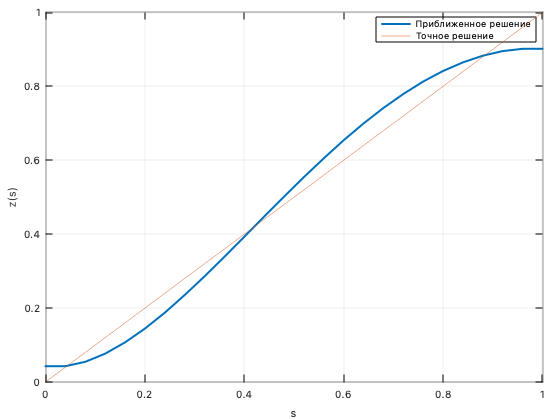
\includegraphics[width=0.7\textwidth]{picture.png}
    \caption{Сравнение точного решения и приближенного решения при $\alpha=0.03$.}
\end{figure}

\subsection{Код программы 2}
\noindent\textit{Моделирование решения с зашумлённой правой частью: $u_\delta(x) = u_T(x) + \delta\cdot\xi$, $\delta=0.01$. Демонстрация влияния случайных погрешностей на решение (без регуляризации).}
\begin{verbatim}
a = 0;
b = 1;
h = 0.01;
delta = 0.01;
x = a:h:b;
s = a:h:b;
N = length(x)

const = 0.5 * (1 - exp(-2));

A = zeros(N, N);
for j = 1:N
  for i = 1:N
    K_val = const * exp(-(x(j) + s(i)));
    A(j, i) = h * K_val;
  end
end

z_true = @(s) s;

u = zeros(N, 1);
for j = 1:N
  sum_val = 0;
  for i = 1:N
    K_val = const * exp(-(x(j) + s(i)));
    sum_val = sum_val + K_val * z_true(s(i));
  end
  u(j) = h * sum_val + delta * rand;
end

z_numeric = A \ u;

z_exact = s';

figure;
plot(s, z_exact, 'b-', 'LineWidth', 2);
hold on;
plot(s, z_numeric, 'ro--', 'LineWidth', 1.5);
xlabel('s');
ylabel('z(s)');
grid on;
\end{verbatim}

\subsection{Результат 2}
\begin{figure}[h!]
    \centering
    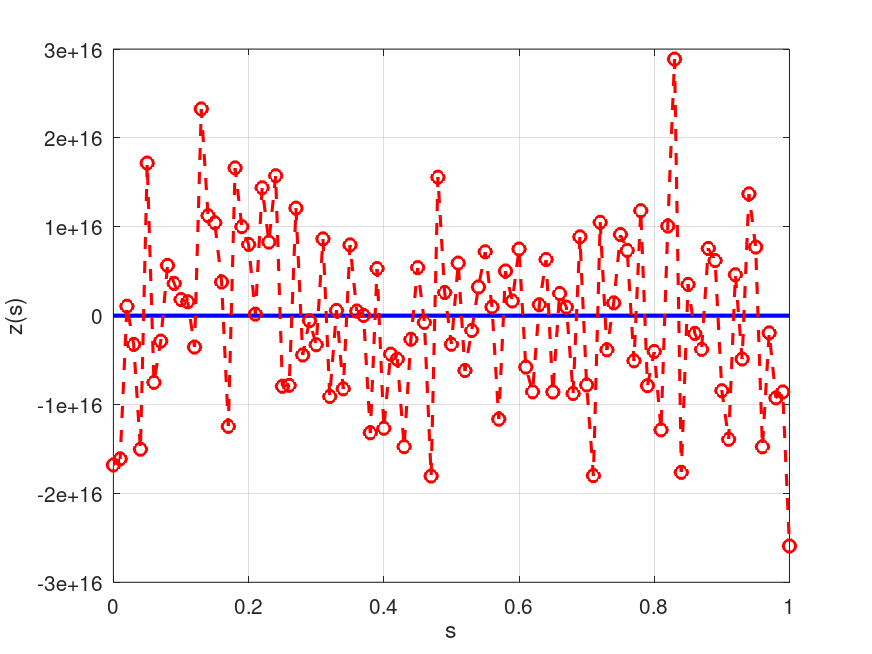
\includegraphics[width=0.7\textwidth]{picture2.png}
    \caption{Решение уравнения с зашумленной правой частью ($\delta=0.01$): точное решение $z_T(s)=s$ и численное решение $z_{\text{num}}(s)$ без регуляризации.}
\end{figure}

\newpage

\begin{thebibliography}{99}
\bibitem{1} Тихонов А.Н., Арсенин В.Я. Методы решения некорректных задач. — 2-е изд. — М.: Наука. Главная редакция физико-математической литературы, 1979. — 288 с.
\end{thebibliography}

\end{document}